\term{Variational programming} \cite{\VPcore} is an emerging paradigm for representing and computing with explicit variation in code and data.
%
It is a generalization of the ideas underlying \term{faceted execution} \cite{\VPfacets} for enforcing dynamic information-flow security and \term{variability-aware execution} \cite{\VPaware} for testing software product lines, and has a range of other applications across computer science such as model checking \cite{Cla10}.
%
However, integrating side effects (e.g. state updates, exceptions, file I/O, standard input/output, and database queries) in variational programs is challenging because the execution environment of these programs is not variational. Therefore, we cannot separate the effect of one variant from the other which causes effects to be performed in wrong contexts (the words effect and side effect are interchangeably used in this thesis).

In this thesis, we argue that \term{algebraic effects} can be used to resolve the problem of combining variation and effects by enabling programmers to extend variational programming environments to handle new kinds of effects or handle existing effects in different ways. We present a proof-of-concept prototype in the \emph{Eff} programming language that demonstrates how the variational programming environment can be extended to support file input/output. 
%

In this chapter, we discuss the insight, formalization, and execution of variational programming. We show the challenge of integrating variational programming with side effects. 
%
We explore various approaches in overcoming these challenges and discuss their limitations.
%
We discuss our solution and its advantages and drawbacks.
%
Finally, we outline the contributions of this work.

A core insight of variational programming is that the execution of sets of related programs, and/or execution over sets of related data, can be made faster by computing over a \emph{single variational artifact} that shares common parts while capturing differences through localized, explicit \emph{variation points}. To illustrate this insight, consider the three related programs which calculate the flight cost for different types of tickets in a booking system and the corresponding \textbf{variational flight cost} program in Figure \ref{fig:vp_eg}. We assume tickets come in three categories: \textbf{Economy}, \textbf{Business} or \textbf{First}. Also, there are \$55 flight fees and a \$45 booking fee added to the cost. In each case, the price is calculated by summing up the price per ticket with the total fees.

\begin{figure}[h]
    \centering
\begin{minipage}[t]{0.49\textwidth}
\textbf{\underline{Economy}} \\
\texttt{let ecoPr =  \$649;;}\\ 
\texttt{let cost = }\\
$\texttt{ \quad 55 + 45 + ecoPr;;} \\$
\end{minipage}
\begin{minipage}[t]{0.49\textwidth}
\textbf{\underline{Business}} \\
\texttt{let busPr =  \$3955;;}\\
\texttt{let cost = }\\
$\texttt{ \quad 55 + 45 + busPr;;} \\$

\end{minipage}
\hfill

\begin{minipage}[t]{0.49\textwidth}
\textbf{\underline{First}} \\
\texttt{let fstPr =  \$5812;;}\\
\texttt{let cost = }\\
$\texttt{ \quad 55 + 45 + fstPr;;} \\$

\end{minipage}
\begin{minipage}[t]{0.49\textwidth}
\textbf{\underline{Variational flight cost}} \\
\texttt{let vTicketPr = }\\ 
$\texttt{ \quad \Chc[\texttt{Economy}]{\texttt{\$649}}{\Chc[\texttt{Business}]{\texttt{\$3955}}{\texttt{\$5812}}}}$\\
\texttt{let vCost = }\\
$\texttt{ \quad 55 + 45 + vTicketPr;;} \\$
\end{minipage}\\

\caption{Variational flight cost.}
  \label{fig:vp_eg}
\end{figure}
%
 The value $\Chc[\texttt{Business}]{\texttt{\$3955}}{\texttt{\$5812}}$ represents a \term{choice} between the alternatives $\texttt{\$3955}$ and $\texttt{\$5812}$ (this choice is nested in another choice). The \term{condition} of the choice is an \term{option} \texttt{Business}, which may be either enabled (true), disabled (false), or open. A choice is similar to a conditional expression (if-then-else), except that if its condition is open, it represents \term{both} alternatives at the same time. Multiple choices with the same condition will always be synchronized while choices with conditions based on different options may vary independently. 
 
Enabling or disabling a choice is what we call \term{selection}. To select the left alternative of the choice \texttt{vTicketPr}, we say (\texttt{selectV Economy vTicketPr}). This returns {\texttt{\$649}}. To select the right alternative of it, we say (\texttt{selectV (!Economy) vTicketPr}). 
%
This returns {\Chc[\texttt{Business}]{\texttt{\$3955}}{\texttt{\$5812}}}. An open selection (\texttt{selectV true vTicketPr}) selects both alternatives, so this returns \texttt{vTicketPr}. The notation and semantics of choices is a previous work on the \term{choice calculus}~\cite{EW11tosem,Walk13thesis,HW16fosd}.

We can extend the evaluation semantics of our programming language to include choices by simply mapping over their alternatives. This allows us to evaluate \texttt{vCost} to the following choice with the following sequence of reduction steps.
%
\begin{align*}
\underline{\texttt{55+45+\Chc[\texttt{Economy}]{\texttt{649}}{\Chc[\texttt{Business}]{\texttt{3955}}{\texttt{5812}}}}}\\
~\Step~ & \texttt{\underline{55+45} + \Chc[\texttt{Economy}]{649}{\Chc[\texttt{Business}]{\texttt{3955}}{\texttt{5812}}}} \\
~\Step~ & \texttt{100 + \underline{\Chc[\texttt{Economy}]{\texttt{649}}{\Chc[\texttt{Business}]{\texttt{3955}}{\texttt{5812}}}}} \\
~\Step~ & \texttt{\Chc[\texttt{Economy}]{\underline{\texttt{649+100}}}{\Chc[\texttt{Business}]{\texttt{3955+100}}{\texttt{5812+100}}}} \\
~\Step~ & \texttt{\Chc[\texttt{Economy}]{\texttt{749}}{\underline{\Chc[\texttt{Business}]{\texttt{3955+100}}{\texttt{5812+100}}}}} \\
~\Step~ & \texttt{\Chc[\texttt{Economy}]{\texttt{749}}{\Chc[\texttt{Business}]{\underline{\texttt{3955+100}}}{\texttt{5812+100}}}}  \\
~\Step~ & \texttt{\Chc[\texttt{Economy}]{\texttt{749}}{\Chc[\texttt{Business}]{\texttt{405}5}{\underline{\texttt{5812+100}}}}}  \\
~\Step~ & \texttt{\Chc[\texttt{Economy}]{\texttt{749}}{\Chc[\texttt{Business}]{\texttt{4055}}{\texttt{5912}}}}
\end{align*}
%
This reduction process represents \term{variational execution} which dynamically evaluates all variants of a program, but observe that we only visited the expression $\texttt{55 + 45}$ once rather than three times if we had evaluated the three programs separately.
%
Although the saving here is small, it adds up as the size of shared programs and the number of independent options increases.
%
In fact, many applications of variational programming involve efficiently computing or exploring an exponential number of variants by exploiting the ideas of capturing variation locally (e.g.\ in choices) and sharing common parts of data and computations. 

\begin{wrapfigure}{r}{0.25\textwidth}
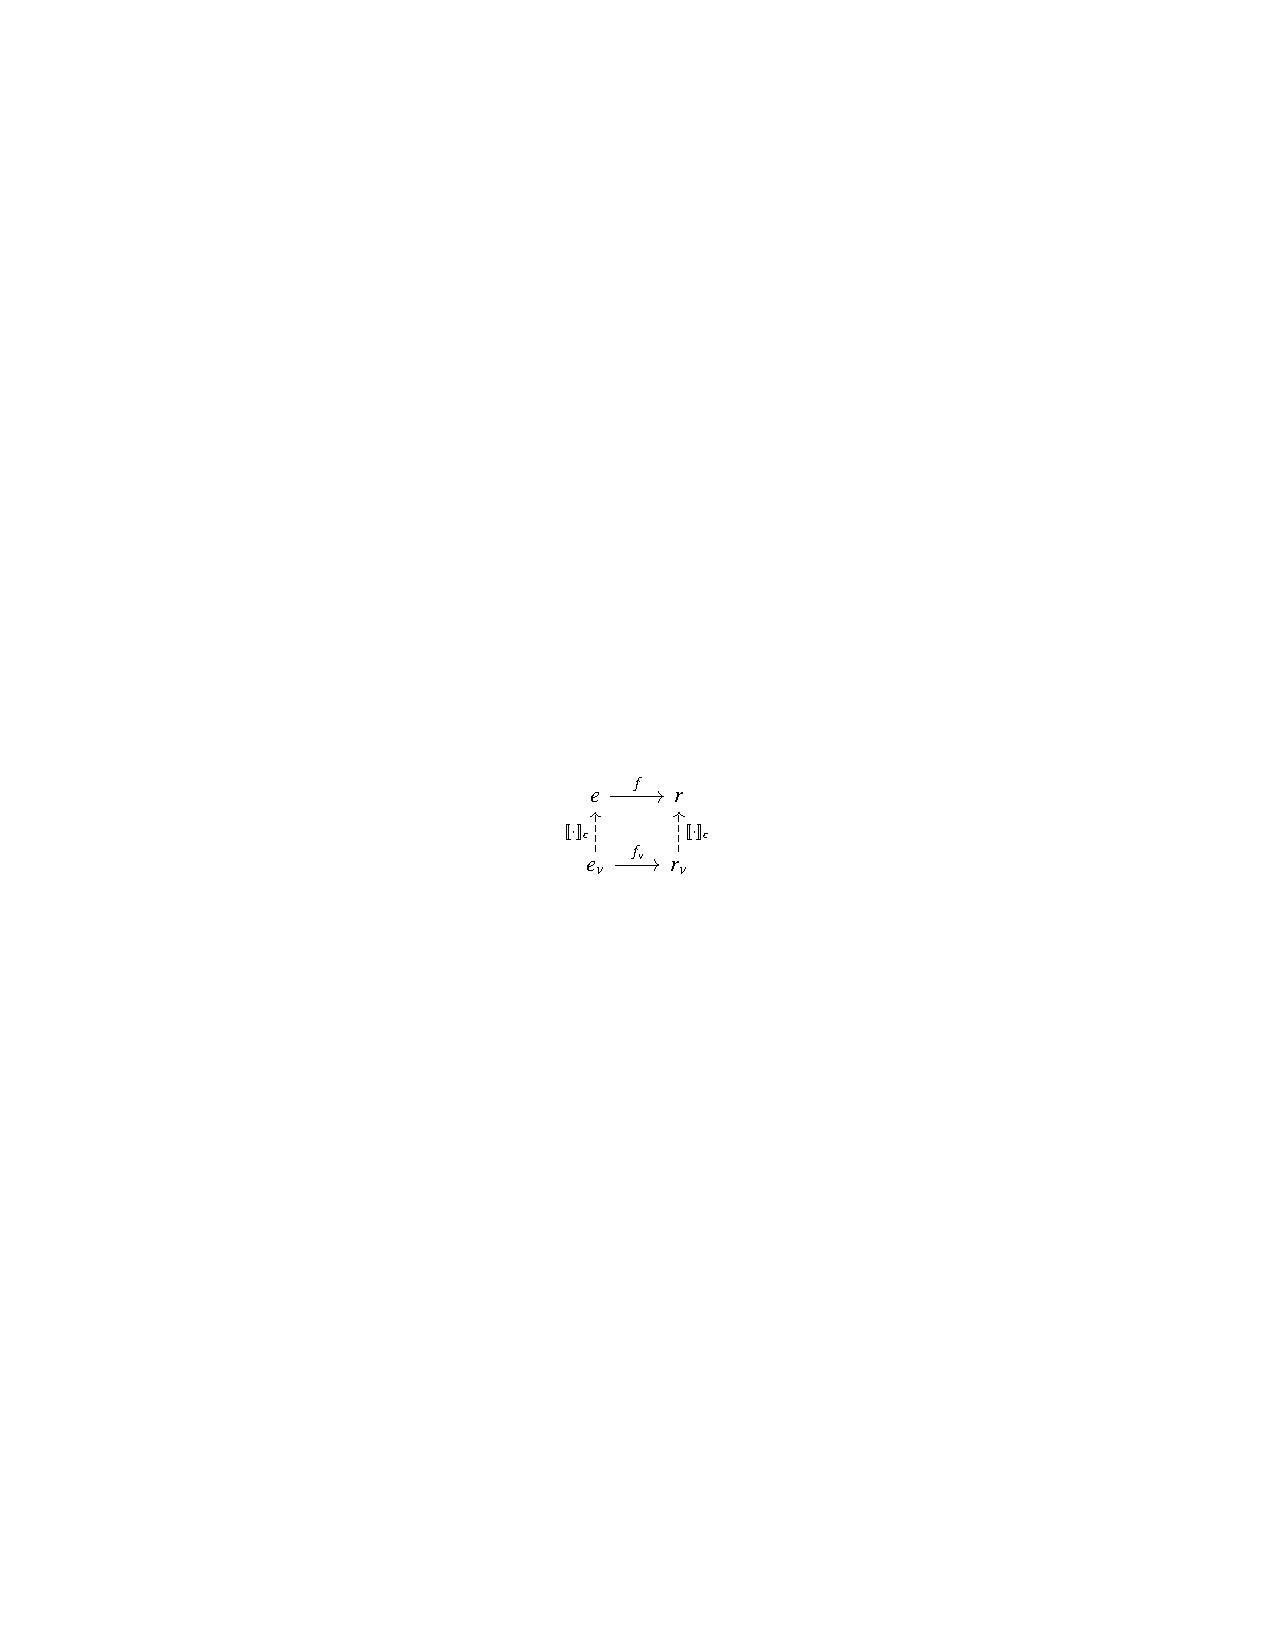
\includegraphics[width=0.9\linewidth]{figures/diagram.pdf} 
\end{wrapfigure}

When mapping analyses or computations over variational terms, the crucial property
that is maintained is \term{variation preservation} \cite{CEW16ecoop}. This is illustrated by the commuting
diagram at right, where \texttt{f} is a plain function that transforms a plain expression \texttt{e} into a plain result \texttt{r}, and $\texttt{f}_\texttt{v}$ is the corresponding \term{variational function} that transforms the variational expression $\texttt{e}_\texttt{v}$ into a variational result $\texttt{r}_\texttt{v}$. The operation $[\![.]\!]_{\texttt{c}}$ refers to the select operation mentioned above; for example, $[\![\texttt{e}_\texttt{v}]\!]_{\texttt{c}}$ is equivalent to \texttt{select c $\texttt{e}_\texttt{v}$ = e}
% selects from  $\texttt{e}_\texttt{v}$ with option \texttt{c}, yielding \texttt{e}. 
The variation-preservation property states that $\texttt{f}_\texttt{v}$ is exactly equivalent to running \texttt{f} on every plain variant of $\texttt{e}_\texttt{v}$. That is, we obtain the same plain result \texttt{r} by either $\texttt{f}([\![\texttt{e}_\texttt{v}]\!]_{\texttt{c}})$ or $[\![\texttt{f}_\texttt{v}(\texttt{e}_\texttt{v})]\!]_{\texttt{c}}$, for any option \texttt{c}.

Now, consider adding side effects to a variational program. For example, someone might like to write the variational flight cost calculated in Figure \ref{fig:vp_eg} into a file as shown below. 
%
\begin{lstlisting}[escapeinside={(*}{*)}]
#WriteFile "flight.txt" ("The total flight cost:");
#WriteFile "flight.txt" ("$" + (* \Chc[\texttt{Economy}]{\texttt{"749"}}{\Chc[\texttt{Business}]{\texttt{"4055"}}{\texttt{"5912"}}}*))
\end{lstlisting}
%
With the current implementation of variational execution, every choice alternative would be visited. Hence, side effects that occur in choices would be performed during the process even in the alternative context. To see how this is an issue, look at the following output of the program above. 
%
\begin{lstlisting}
The total flight cost: 
$749
4055 
5912
\end{lstlisting}
%
This program writes the text of each variant while the desired behavior is to only write the text of the corresponding variant. Variational programming uses variational data-structures to manage different variants and separate their results, but the current environments of the effects we work with are not variational, so we can not separate their variants which causes this problem.

There are several solutions to allow working with side effects in variation. One possible solution is to make a variation-aware interface for every effect type we work with, that is a variational file system, database \cite{ATW17dbpl} and so on. Thus, if the file system was variational, there would be conceptually a different file instance for every new option introduced by a choice as shown below.\\

\begin{minipage}{0.3\textwidth}
\textbf{\underline{Economy.txt}} \\
\texttt{The total flight cost: }\\
\texttt{\$749}\\
\end{minipage}
\begin{minipage}{0.3\textwidth}
\textbf{\underline{NotEconomyBusiness.txt}} \\
\texttt{The total flight cost: }\\
\texttt{\$4055}\\
\end{minipage}
\begin{minipage}{0.3\textwidth}
\textbf{\underline{NotEconomyNotBusiness.txt}} \\
\texttt{The total flight cost: }\\
\texttt{\$5912}\\
\end{minipage}\\
\hfill\\
%
As we introduce more options, more instances should be created. However, making a special variational infrastructure for every effect type is very complex, infeasible or incompatible in some domains. Another solution is to avoid variational execution from running side effects when they occur in variation, but this would cut their useful applications.
% Therefore, we propose a library level solution which allows programmers to work with effects in variational programs.

In this thesis, we argue that algebraic effects can be used to resolve the problem of combining variation and effects by enabling programmers to flexibly and incrementally extend variational programming environments to handle new kinds of effects or handle existing effect differently. We present a proof-of-concept prototype in the \emph{Eff} programming language. We implement variation as an algebraic effect and then demonstrate how the variational programming environment can be extended to support file input/output. Given that there is not a comprehensive solution for all effects, this approach is the best given the constraints. It allows programmers to work with effects on a case-by-case basis by building new libraries to handle them. Unfortunately, implementing variation as an effect is not efficient as the number of options increases. Therefore, we argue that having built-in features in the programming language itself for working with variation would be more effective.

This work includes the following contributions. 
%
\begin{itemize}
  \item We implement variation as an effect and show examples of how it works (Chapter \ref{sec:Variational_exe}). We show the limitations of this implementation when we start to integrate side effects in variational programs (Chapter \ref{sec:Variational_effects}). Our approach in addressing these limitations is by writing new handlers for the variation effect to work with interaction of variation and effects on a case-by-case basis using algebraic effects. As a proof-of-concept, we write new handlers to support file writing (Chapter \ref{sec:file_IO_writing}) and reading (Chapter \ref{sec:file_IO_reading}) which are hard to work with otherwise. As part of this, we also extend text files with a variation encoding (Chapter \ref{sec:file_format}).
  \item We introduce an abstract variational queue that can be used in different variational programming applications (Chapter \ref{sec:queue_lib}). We use the variational queue to represent variational files as part of our proof-of-concept. 
  \item We discuss the limitations of implementing variation as an effect (Chapter \ref{sec:efficiency}).
\end{itemize}
Our prototype implementation is publicly available at the GitHub repository VEffect\footnote{https://github.com/lambda-land/VEffect}. 

